
%%% Local Variables: 
%%% mode: latex
%%% TeX-master: "lista1"
%%% End: 
\documentclass[11pt,epsf]{report}
\setlength{\vsize}{297mm}
\setlength{\hsize}{210mm}
\setlength{\textheight}{230mm}
\setlength{\textwidth}{170mm}
%\voffset -2.5cm
\hoffset -2.5cm

\usepackage[latin1]{inputenc}
%\usepackage{latexsym}
%\usepackage{amssymb}
\usepackage[dvips]{graphicx}

\newenvironment{alternativas}{\renewcommand{\labelenumi}{(\alph{enumi})}\begin{enumerate}\addtolength{\itemsep}{-2.5mm}\setlength{\parsep}{0pt}}{\end{enumerate}}

\newcounter{qcounter}
\newenvironment{question}{\stepcounter{qcounter}\paragraph{\arabic{qcounter}.}}{}




\begin{document}

\begin{center}
ENG04035 - Sistemas de Controle I \\
 Prof. Jo�o Manoel Gomes da Silva Jr. e Romeu Reginatto \\
Comportamento em Regime Permanente de Sistemas de Controle Realimentados
\end{center}





\begin{enumerate}

\item Determine os coeficientes de erro estacion\'{a}rio $k_{p}$ e $k_{v}$ 
e o erro em regime permanente da resposta a excita\c{c}\~{o}es do tipo
degrau e rampa para os sistemas abaixo. Procure entender
a influ\^{e}ncia do par\^{a}metro $k$ no erro em regime permanente. 

\begin{flushleft}
\setlength{\unitlength}{1.5mm}
\begin{picture}(100,36)(0,0)
\put(0,30){(a)}
\put(5,30){\vector(1,0){12}}
\put(19,30){\circle{4}}
\put(21,30){\vector(1,0){12}}
\put(33,26){\framebox(12,8){\mbox{\large $\frac{5}{s+2}$}}}
\put(45,30){\vector(1,0){16}}
\put(53,30){\line(0,-1){12}}
\put(53,18){\vector(-1,0){8}}
\put(33,14){\framebox(12,8){\mbox{\large $k$}}}
\put(33,18){\vector(-1,0){12}}
\put(19,18){\circle{4}}
\put(19,20){\vector(0,1){8}}

\put(61,26){\framebox(20,8){\mbox{\large $\frac{8(s+2)}{(s+1)(s+3)}$}}}
\put(81,30){\vector(1,0){12}}
\put(87,30){\line(0,-1){20}}
\put(87,10){\line(-1,0){68}}
\put(19,10){\vector(0,1){6}}

\put(8,31){R(s)}
\put(88,31){Y(s)}
\put(16,28){\mbox{\tiny $+$}}
\put(17,26){\mbox{\tiny $-$}}
\put(20,15){\mbox{\tiny $+$}}
\put(21.5,16){\mbox{\tiny $+$}}
\end{picture}
\end{flushleft}



\begin{flushleft}
\setlength{\unitlength}{1.5mm}
\begin{picture}(85,30)(0,0)
\put(0,20){(b)}
\put(5,20){\vector(1,0){12}}
\put(19,20){\circle{4}}
\put(21,20){\vector(1,0){12}}
\put(33,16){\framebox(12,8){\mbox{\large $\frac{8}{s(s+3)}$}}}
\put(45,20){\vector(1,0){16}}
\put(53,20){\line(0,1){12}}
\put(53,32){\vector(-1,0){8}}
\put(33,28){\framebox(12,8){\mbox{\large $\frac{ks}{s+20}$}}}
\put(33,32){\line(-1,0){14}}
\put(19,32){\vector(0,-1){10}}

\put(61,16){\framebox(12,8){\mbox{\large $\frac{1}{s+2}$}}}
\put(73,20){\vector(1,0){12}}
\put(79,20){\line(0,-1){10}}
\put(79,10){\line(-1,0){60}}
\put(19,10){\vector(0,1){8}}
\put(8,21){R(s)}
\put(80,21){Y(s)}
\put(16,18){\mbox{\tiny $+$}}
\put(17,16){\mbox{\tiny $-$}}
\put(17,24){\mbox{\tiny $-$}}
\end{picture}
\end{flushleft}



\item
Seja a fun\c{c}\~{a}o de transfer\^{e}ncia de um sistema de controle com
realimenta\c{c}\~{a}o unit\'{a}ria dada por:
\[
T(s)=\frac{Y(s)}{R(s)}=\frac{b_{m}s^{m}+b_{m-1}s^{m-1}+\cdots+b_{1}s+b_{0}}
           {s^{n}+a_{n-1}s^{n-1}+\cdots+a_{1}s+a_{0}}
\]
Determine express\~{o}es para obter o erro em regime permanente para entradas
do tipo degrau e rampa em fun\c{c}\~{a}o dos par\^{a}metros
de $T(s)$. Determine, tamb\'{e}m, express\~{o}es para os coeficientes de
erro de posi\c{c}\~{a}o e velocidade.


\item
A partir dos resultados do item 2, esbo\c{c}e a resposta dos sistemas
abaixo para a excita\c{c}\~{a}o ilustrada na figura~\ref{rr}.

\[ (a)\,\,\,\, T(s)=\frac{200}{(s+20)(s+10)(s+1)}   \]

\[ (b)\,\,\,\, T(s)=\frac{25(s+4)(s+8)}{s^4+25s^3+180s^2+300s+800} \]

\begin{figure}
\begin{center}
\setlength{\unitlength}{1.5mm}
\begin{picture}(55,25)(0,0)
\put(4,5){\vector(1,0){50}}
\put(5,4){\vector(0,1){20}}
\put(5,10){\line(1,0){15}}
\put(20,10){\line(2,1){15}}
\put(35,17.5){\line(1,0){15}}
\put(20,4){\line(0,1){2}}
\put(35,4){\line(0,1){2}}
\put(4,10){\line(1,0){2}}
\put(4,17.5){\line(1,0){2}}
\put(19,2){50}
\put(33,2){100}
\put(54,2){t(s)}
\put(2,9){2}
\put(2,17){5}
\put(0,23){r(t)}
\end{picture}
\end{center}
\caption{Entrada de Refer\^{e}ncia para o Problema 3}
\label{rr}
\end{figure}


\item
Para o sistema abaixo, determine $T_i$ que faz com que o sistema
apresente erro em regime permanente, em resposta a rampa unit\'{a}ria,
igual a $0.1$. 

\begin{center}
\setlength{\unitlength}{1.5mm}
\begin{picture}(76,26)(0,0)
\put(0,20){\vector(1,0){10}}
\put(12,20){\circle{4}}
\put(14,20){\vector(1,0){10}}
\put(24,16){\framebox(10,8){\mbox{\large $\frac{1}{T_i\,s}$}}}
\put(34,20){\vector(1,0){12}}
\put(46,16){\framebox(20,8){\mbox{\large $\frac{20}{(s+2)(s+10)}$}}}
\put(66,20){\vector(1,0){10}}
\put(70,20){\line(0,-1){10}}
\put(70,10){\line(-1,0){58}}
\put(12,10){\vector(0,1){8}}
\put(2,21){R(s)}
\put(70,21){Y(s)}
\put(9,18){\mbox{\tiny $+$}}
\put(10,17){\mbox{\tiny $-$}}
\end{picture}
\end{center}



\item
Para cada uma das perturba\c{c}\~{o}es $Q_1(s)$ a $Q_4(s)$ do sistema abaixo,
determine se \'{e} ou n\~{a}o rejeitada assintoticamente (justifique suas 
respostas) considerando perturba\c{c}\~{o}es tanto do tipo degrau quanto rampa.

\begin{center}
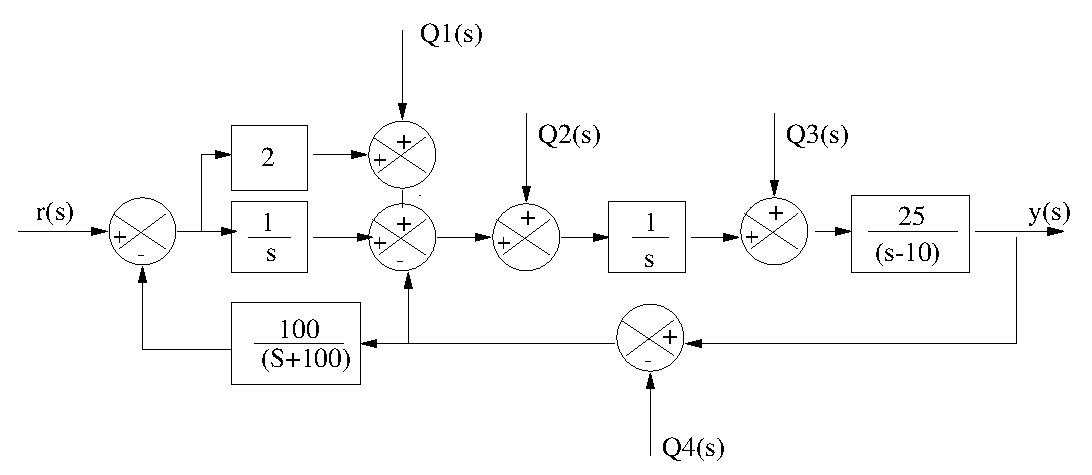
\includegraphics[width=10cm]{pert.eps}
\end{center}



\item Considere o sistema da figura abaixo. Assuma que a din�mica do 
sensor � dada por $H(s)=1$.
     \begin{itemize}
        \item[a)] O sistema pode seguir uma refer�ncia $r$ do tipo 
                  degrau com erro  nulo  em regime permanente? Justifique.
        \item[b)] Pode o sistema rejeitar perturba��es $w$ do tipo degrau?
Justifique.
        \item[c)] Esboce o gr�fico de $u(t)$, $e(t)$ e $y(t)$ considerando a 
aplica��o de um degrau de amplitude $1.5$ em $r$ e, $20$ segundos ap�s,
a a��o de uma perturba��o $w$ do tipo degrau de amplitude $-0.3$.
        \item[d)] Repita a), b) e c) considerando $H(s)=\frac{5}{(s+20)}$
     \end{itemize}

\begin{center}
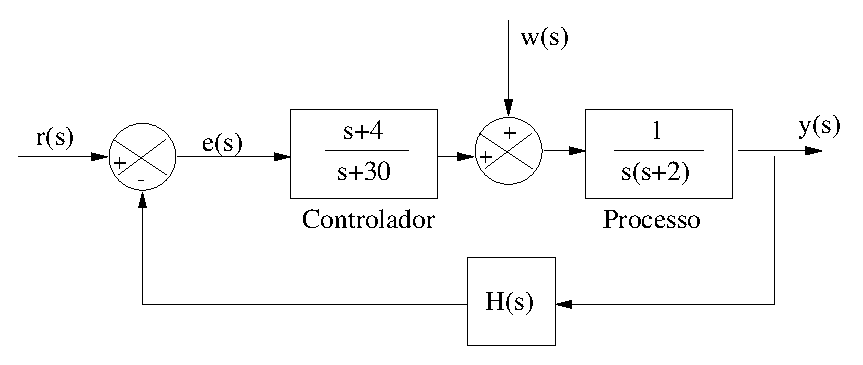
\includegraphics[width=10cm]{sens.eps}
\end{center}

        
\item Considere os dois sistemas abaixo:

\begin{center}
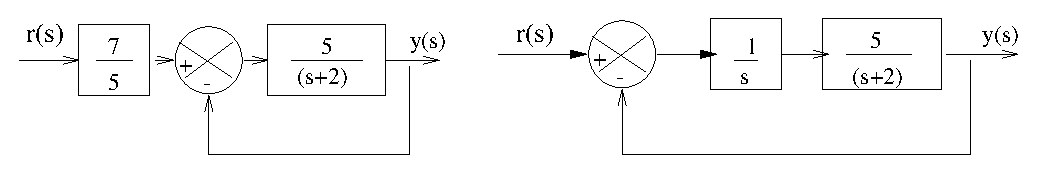
\includegraphics[width=10cm]{robus.eps}
\end{center}

\begin{itemize}
       \item[a)] Mostre que os dois sistemas s�o capazes de seguir 
refer�ncias $r$ constantes com erro nulo em regime permanente.
       \item[b)] Analise as diferen�as entre os dois sistemas com 
respeito a:
          \begin{itemize}
             \item robustez ao seguimento da refer�ncia se os par�metros
da planta variam (i.e. os dois sistemas continuam seguindo a refer�ncia 
com erro nulo ?) 
             \item estabilidade relativa e comportamento din�mico
 do sistema em malha fechada.
          \end{itemize}
\end{itemize}


\item Considere o seguinte diagrama em blocos:

\begin{center}
\includegraphics[width=8cm]{smf_ct_pl.eps}
\end{center}

\begin{enumerate}
\item Que condi��es devem ser satisfeitas para que seja 
poss�vel seguir uma refer�ncia senoidal, com freq��ncia 
angular $w$rad/s, com erro nulo em regime permanente.

\item Que condi��es devem ser satisfeitas para que seja 
poss�vel rejeitar assintoticamente em regime permanente
uma refer�ncia senoidal, com freq��ncia 
angular $w$rad/s?      
\end{enumerate}         

\end{enumerate}




\end{document}











